\chapter{Opis projektnog zadatka}
		
		\textbf{\textit{dio 1. revizije}}\\
		
		Cilj ovog projekta je razviti programsku podršku za stvaranje web aplikacije „Nestali ljubimci“ koja će korisniku omogućiti pregledavanje, pretragu i objavljivanje oglasa o nestalim kućnim ljubimcima, kao i pružiti resurse za kontaktiranje skloništa za životinje i druge korisnike u svrhu pronalaženja izgubljenih ljubimaca, bilo da se radi o vlastitom ili tuđem ljubimcu. Ovom web aplikacijom smanjit će se pojava nepraktičnog oglašavanja nestanaka, opažanja i pronalaska s preciznim podacima kućnih ljubimaca koja se danas vrlo često može pronaći na raznim internetskim platformama poput društvenih mreža, stranica za oglašavanje, foruma itd. Web aplikacija će biti intuitivna i korisna, pružajući vlasnicima kućnih ljubimaca, skloništima za životinje i ostalim uključenim osobama pomoć u rješavanju ovih stresnih situacija. Dodatno, web aplikacija će biti optimizirana za mobilne uređaje kako bi pružila korisnicima najbolje iskustvo. Ovakav razvoj web aplikacije pružit će svim dionicima brži pristup i reakciju, što često igra ključnu ulogu u uspješnom završetku potrage za izgubljenim kućnim ljubimcem.
		
		Prilikom pokretanja sustava prikazuju se oglašeni nestali kućni ljubimci i skloništa za životinje.
		
		Neregistrirani korisnik ima pristup funkcionalnosti pretraživanja oglašenih nestalih kućnih ljubimaca prema raznim kategorijama podataka o ljubimcu, kao i pretraživanju skloništa za životinje putem naziva skloništa. Pretraživanje nestalih kućnih ljubimaca prema kategorijama obuhvaća sljedeće informacije o ljubimcu: vrstu, ime na koje se ljubimac odaziva, datum i vrijeme nestanka, lokaciju nestanka (s korištenjem vanjske usluge za geolociranje, kao što je OpenStreetMap), boju, starost, tekstualni opis i do tri slike ljubimca. Sve navedene kategorije o nestalom ljubimcu mogu se detaljnije pregledati klikom na određeni oglas. Osim ovih podataka, oglas sadrži i kontakt podatke korisnika koji se automatski povlače iz korisničkih podataka danih pri registraciji (poput e-pošte, telefona te posebno za skloništa - naziv skloništa). Dodatno, odabirom određenog kućnog ljubimca omogućava se detaljniji uvid u informacije o njemu, kao i pregled komunikacije vezane uz potragu za ljubimcem. Neregistriranom korisniku je omogućeno prijavljivanje u sustav s postojećim računom (potrebno je upisati korisničko ime i lozinku) ili kreiranjem novog računa. Za kreiranje novog računa potrebni su sljedeći podaci:
		
		\begin{packed_item}
			\item korisničko ime
			\item lozinka
			\item ime
			\item prezime
			\item broj telefona
			\item e-pošta
		\end{packed_item}
		
		Registracijom u sustav, korisniku se dodjeljuju prava registriranog korisnika a naknadno mu se mogu dodijeliti prava skloništa za životinje. Prava registriranog korisnika uključuju sva prava neregistriranog korisnika, te dodatno:
		
		\begin{packed_item}
			\item postavljanje oglasa o nestalom kućnom ljubimcu
			\item uklanjanje oglasa o nestalom kućnom ljubimcu
			\item izmjena oglasa o nestalom kućnom ljubimcu
			\item sudjelovanje u komunikaciji oko potrage za ljubimcem
		\end{packed_item}
		
		Ako registrirani korisnik odluči postaviti oglas obavezan je unijeti niz kategorija podataka o ljubimcu, uključujući vrstu, ime na koje se ljubimac odaziva, datum i vrijeme nestanka, lokaciju nestanka (uz korištenje vanjske usluge za geolociranje, poput OpenStreetMap-a), boju, starost, tekstualni opis i do tri slike. Registrirani korisnici imaju mogućnost komunikacije putem poruka u svrhu potrage za izgubljenim ljubimcem. Poruke mogu sadržavati tekst, slike i geolokaciju (putem vanjske usluge), uz jasno istaknute kontakt informacije korisnika. Registrirani korisnik može ukloniti oglas koje je postavio. Ako korisnik ukloni svoj oglas, taj oglas i sva njegova komunikacija nestati će iz popisa vidljivih oglasa, međutim, oglas će i dalje ostati sačuvan u bazi podataka. Registriranim korisnicima omogućeno je uređivanje oglasa s mogućnošću izmjene svih kategorija podataka, uključujući promjenu kategorije oglasa. Raspoložive kategorije oglasa uključuju:
		
		\begin{enumerate}
			\item ljubimac je nestao i traga se za njim
			\item ljubimac je sretno pronađen
			\item ljubimac nije pronađen i za njim se više aktivno ne traga
			\item ljubimac je pronađen u nesretnim okolnostima
		\end{enumerate}
		
		Svaka izmjena kategorije oglasa u onu koja nije da se za ljubimcem aktivno traga prebacuje oglas automatski u popis neaktivnih oglasa, koji mogu pretraživati samo registrirani korisnici.
		
		Skloništa za životinje su specijalni tip registriranih korisnika koji, osim funkcionalnosti koji imaju ostali registrirani korisnici, imaju dodatnu mogućnost oglašavanja životinja koje su pronašli i koje se nalaze u njihovom prostoru. Takvi oglasi imaju dodatnu kategoriju – u skloništu, pa bi njihove kategorije oglasa bile:
		
		\begin{enumerate}
			\item ljubimac je nestao i traga se za njim
			\item ljubimac je sretno pronađen
			\item ljubimac nije pronađen i za njim se više aktivno ne traga
			\item ljubimac je pronađen u nesretnim okolnostima
			\item ljubimac je u skloništu
		\end{enumerate}
		
		Ova web aplikacija podržava tri tipa korisnika te u aplikaciji nema podržane uloge administratora koji bi se trebao brinuti o administraciji podataka(oglasa, registracije i korisničkih podataka). Prema razini ovlasti koju imaju u web aplikaciji, korisnici su podijeljeni u tri kategorije, rangirane od najviše razine ovlasti do najniže razine ovlasti:
		
		\begin{enumerate}
			\item skloništa za životinje
			\item registrirani korisnici
			\item neregistrirani korisnici
		\end{enumerate}
		
		Svaka registracija korisnika i njihovih korisničkih podataka biti će zabilježena je u bazi podataka, s naglaskom na jedinstvenost korisničkih imena i korisničkih podataka. To znači da neće biti moguće imati dva korisnika s istim korisničkim imenom ili e-poštom. Ova jedinstvenost također se primjenjuje na skloništa za životinje. Sustav će podržavati rad više korisnika u stvarnom vremenu.
		
		Ova web aplikacija pružit će značajnu korist svim vlasnicima kućnih ljubimaca. Svojim funkcionalnostima ne samo da će povećati šanse za pronalazak izgubljenih ljubimaca, već će povezati i sve druge ljude koji imaju jednak cilj, a to je pronalazak izgubljenih ljubimaca. Svi smo svjesni da je gubitak ljubimca izuzetno emotivno zahtjevan događaj. Ovim projektom teži se pronalasku rješenja koje će smanjiti stresne situacije i pružiti podršku osobama koje se nalaze u potrebi da pronađu svoje izgubljene ljubimce. Naglašavamo da će svaki pokušaj zloupotrebe web aplikacije biti strogo kažnjen, s potencijalnim dodatnim sankcijama ako se to smatra potrebnim.
		
		Do sada nije postojala jasna i učinkovita web aplikacija za pronalazak nestalih ljubimaca, već samo postoje neka potencijalna i neučinkovita rješenja poput foruma, oglasnih stranica ili pak društvenih stranica. Neka od tih rješenja prikazana su u nastavku.
	
		\begin{figure}[H]
			\centering
			
\includegraphics[scale=0.3]{slike/Facebook-nestaliLjubimci.PNG}
			\caption{Facebook}
			\label{fig:promjene}
		\end{figure}
	
		\begin{figure}[H]
			\centering
			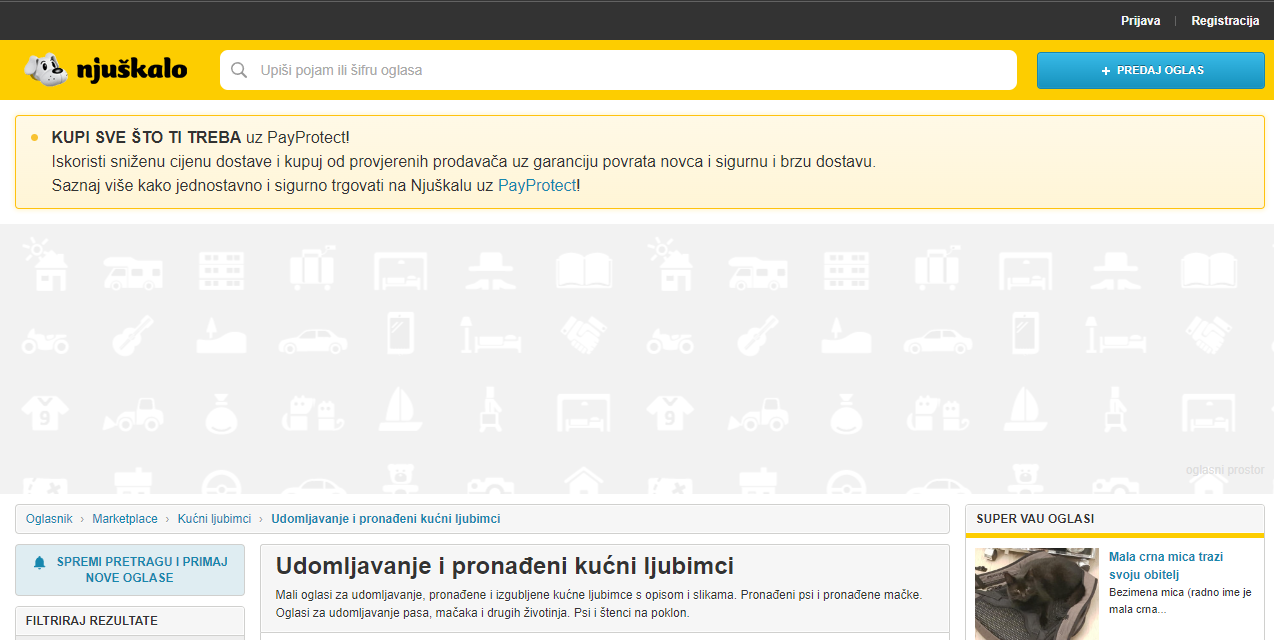
\includegraphics[scale=0.3]{slike/Njuskalo-nestaliLjubimci.PNG}
			\caption{Njuškalo}
			\label{fig:promjene}
		\end{figure}
		
		Web aplikacija za pronalazak nestalih ljubimaca će predstavljati puno učinkovitije rješenje u kojem će se korisnici lako i brzo snalaziti. Dodatno, važno je istaknuti da će svaki oglas za izgubljenog ljubimca, zajedno s odgovarajućom komunikacijom, biti tretiran kao samostalna i odvojena cjelina, bez međusobnih preklapanja s drugim oglasima. Ovim pristupom će biti osigurana jednostavna i brza pretraga unutar objavljenih oglasa, što će rezultirati znatno poboljšanom učinkovitošću i brzinom u usporedbi s tradicionalnim platformama poput Facebooka ili Njuškala.
		
		Prilagodbe rješenja i nadogradnje projektnog zadatka bit će moguće u budućnosti, uz naglasak na korisničkom zadovoljstvu i njihovim mišljenjima. Korisnike se potiče da iznose svoja moguća rješenja i sugestije kako bi se unaprijedila web aplikacija te postala sve korisnija, učinkovitija i uspješnija u pomoći korisnicima u potrazi za izgubljenim ljubimcima.
		
		\eject
		
		
	